% !TeX root = ../main.tex

\chapter{文獻回顧}

本章為文獻回顧,在對整合風力發電與電動汽車的虛擬電廠參與電力市場交易收益模型的建構與分析之前,需要對虛擬電廠、風力發電、電動汽車…等所涉及的領域進行文獻回顧。以下將研究過程中蒐集的文獻經整理後分為虛擬電廠概念、虛擬電廠應用、風電預測評估、電動汽車電池部分進行陳述。

\section{虛擬電廠概念}

由於再生能源的間歇性與隨機性會導致電力供給與需求兩側失衡,學者們提出了整合分散式能源(Distributed Energy Resources, DERs)、儲能設備(Battery Energy Storage System, BESS)與電動汽車(Battery Electric Vehicle, BEV)的虛擬電廠(Virtual Power Plant, VPP)概念。

目前學術上並未對虛擬電廠有統一的定義 \cite{setiawan2007concept}:文獻 \cite{Asmus2010} 中指稱虛擬電廠為依賴於資訊系統,透過網路通訊技術遠端控制電力系統,實現自動輸配電、需量反應與能量儲存…等行為的整合網路;文獻 \cite{Pudjianto2007, Pudjianto2017} 將虛擬電廠分為技術與市場兩大部分,技術層面為提供電力來源的分散式發電,市場層面進行電力市場的交易與管理;文獻 \cite{braun2008review} 將虛擬電廠定義分為控制與通訊兩大單位,前者以直接集中控制方式整合分散式能源,後者透過資通訊系統整合主動用電用戶網路。

綜合上述文獻,虛擬電廠可以視為是一個具備調度發電設備、整合用戶需求的中央控制中心,其概念如圖 \ref{figure: Virtual Power Plant} 所示。其中發電設備可以包括火力發電和核能發電等傳統發電技術,也可以包括風力發電、太陽能發電等再生能源發電技術;透過資訊設備進行發電數量預測、電力價格預測、電力需求預測…等,進行需量反應管理需求面。

\begin{figure}[htbp]
  \centering
  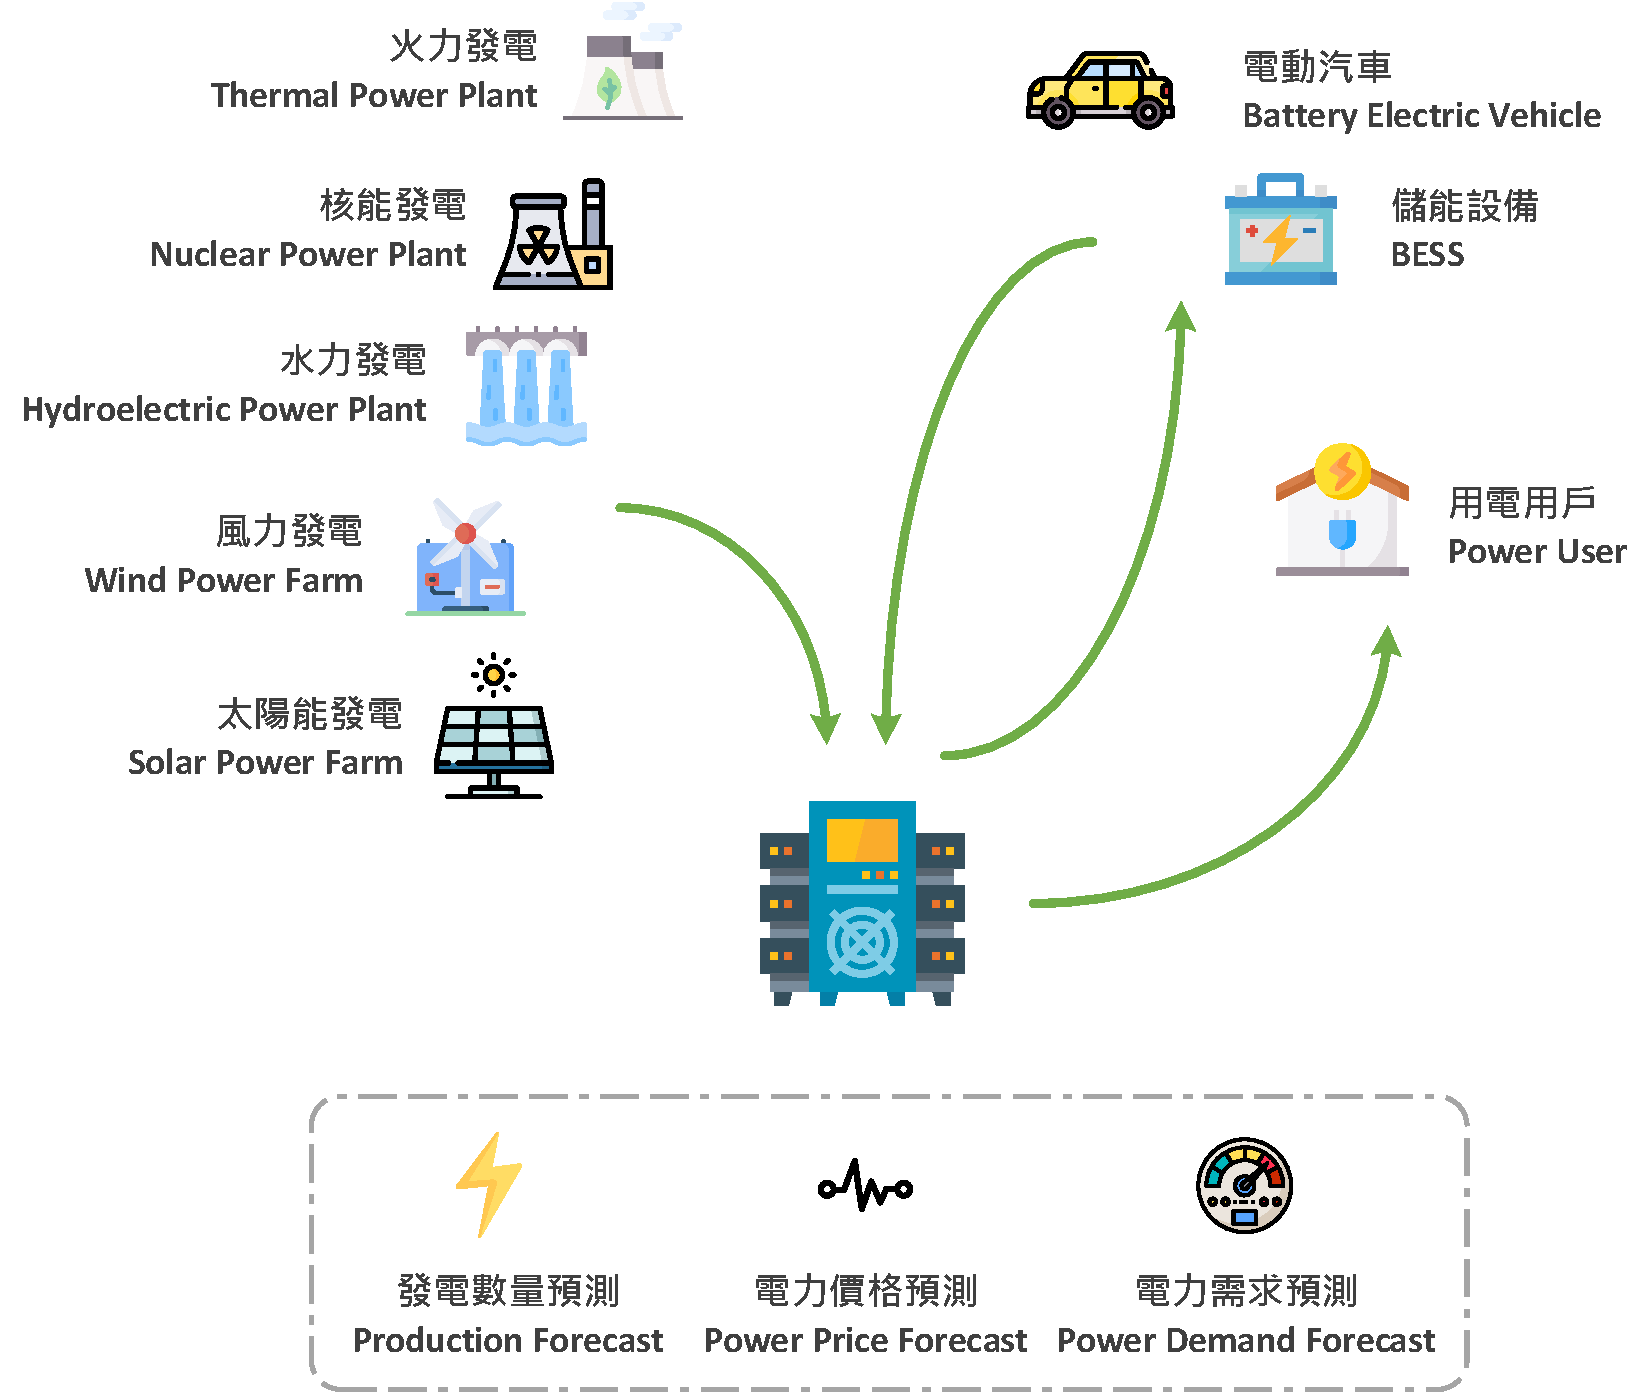
\includegraphics[width=\textwidth]{Virtual Power Plant}
  \caption{虛擬電廠概念}
  \label{figure: Virtual Power Plant}
\end{figure}

\section{虛擬電廠應用}

目前我國採用虛擬電廠概念進行應用與研究的相關文獻並不多,其中文獻 \cite{U0001-2906201000281800} 應用虛擬電廠之概念探討我國電力消費型態改變是否可以減少電力使用所造成的環境衝擊,採用了生命週期評估方法量化涵蓋人體毒性、水體優養化與全球暖化…等在內的八類環境衝擊項目,發現應用虛擬電廠策略後造成的電力消費型態改變可以減少因電力消費所造成之環境衝擊;文獻 \cite{U0027-0212201417510382} 提出虛擬電廠在自由電力市場中的獲利模型並分析其獲利關鍵因素,利用 IEEE 37 母線測試饋線進行最佳電力潮流(Optimal Power Flow)模擬,發現變壓器供電上限和儲能電池設備為虛擬電廠營運商獲利的關鍵因素;文獻 \cite{U0027-2501201611000959} 應用虛擬電廠概念整合太陽光電與電池儲能設備,並採用時間電價與需量反應概念,探討不同用戶負載情境下虛擬電廠的調度狀況,發現儲能設備的調度與時間電價有關且用戶類型不會影響儲能設備調度結果。
文獻 \cite{chung2016vpp} 考慮表燈用戶、高壓用戶與整體社會參與虛擬電場運作時的經濟效益與機會成本,透過量化經濟效益模型評估不同用戶群體參與虛擬電廠是否具備經濟可行性,依據實證分析結果發現鼓勵電力用戶參與彈性電價方案有助於節省容量成本並具減碳效益,並提出政府應扶植虛擬電廠產業在我國發展、未來整體電力系統政策應具備跨系統配套方案…等政策論點。

\section{風電預測評估}

風力發電是目前再生能源發電中相對成熟的技術,如何對風速與風能進行預測與評估是風力發電項目可行性研究與輸配電網規劃研究的重要工作之一。依據歷年風速與風向資料進行的風力發電效益評估,根據時間尺度與應用層面的不同,可以分為長期風能評估(Wind Resource Assessment)與短期風能預測(Wind Energy Forecasting),長期風能評估用來評估一個地區是否有足夠潛力發展風力發電;而短期風能預測則用於電力系統中的調度規劃。

長期風能評估方面,多以一般統計方法將歷史風速資料與機率分布函數進行擬和,並透過風力機組的功率曲線轉換成對應的風能分布,用以評估潛在風能。目前已有許多學者投入相關研究,其中最早由文獻 \cite{justus1976nationwide} 提出透過不同的機率密度函數描述風速,評估潛在風能的方法;文獻 \cite{nigim2007heuristic, panda1990stochastic, kumar2019wind} 採用機率分布函數擬合風速,分別評估加拿大和印度不同地區的潛在風能,作為風場選址考量;文獻 \cite{chuang2001wind} 分別就臺灣地區過往四十年間的平時風速與極值風速探討其適用機率分布,發現韋伯機率函數可用於描述平時風速,與文獻 \cite{teyabeen2015statistical} 針對利比亞地區所進行的統計分析結果一致。

短期風能預測方面,目前多採時間序列方法觀察過去風速數據中隱含的趨勢,並針對風力電場進行風能預測,建立模型以預測未來風速。傳統時間序列預測的模型建構方法,根據平穩性條件可以分為應用於平穩時間序列的自迴歸模型(Auto Regressive Model, AR Model)、移動平均模型(Moving Average Model, MA Model)與自迴歸移動平均模型(Auto Regressive Moving Average Model, ARMA Model),以及應用於非平穩時間序列的差分自迴歸移動平均模型(Auto Regressive Integrated Moving Average Model, ARIMA Model);近年來也有不少研究致力於將機器學習方法中的人工神經網路(Artificial Neural Network
, ANN)與支持向量迴歸(Support Vector Regression, SVR)應用於時間序列預測。除此之外,為了更加準確地分析非平穩時間序列,通常會將時間序列進行分解,常見有以下分解方法:

\begin{itemize}
  \item \textbf{趨勢分解 (Trend Decomposition)} :依據季節性將時間序列模型分解為週期分量(seasonal component)、趨勢分量(trend component)與殘留分量(remainder component),再與實際數據進行擬合求解模型參數,即 STL 分解(Seasonal-Trend Decomposition Based on Loess)。 \cite{cleveland1990stl}
  \item \textbf{訊號分解(Signal Decomposition)}:將時間序列透過訊號處理方式分解為高頻訊號與低頻訊號,分別進行模型擬合後將預測值進行疊合。常見訊號分解方法有傅立葉轉換(Fourier Transform, FT)、小波轉換(Wavelet Transform, WT)與經驗模態分解(Empirical Mode Decomposition, EMD)…等。 \cite{foster1996wavelets}
\end{itemize}

相關研究中,文獻 \cite{liu2012comparison} 提出 ARIMA-ANN 模型與 ARIMA-Kalman 模型來預測短期風速,比較後顯示兩者皆均具有良好的性能可以用於非固定風速預測;文獻 \cite{kusiak2009short} 採用機器學習方法中的支持向量迴歸模型(SVR Model)、多層感知器模型(MLP Model)與決策樹模型進行預測並比較其準確性,其中以支持向量迴歸模型的誤差最小;文獻 \cite{hu2013hybrid} 提出結合 EEMD 與 SVM 的組合模型進行風速預測,並以中國西北\uline{酒泉}地區數據進行驗證,發現相較於傳統時間序列預測方法具有更高的準確性;文獻 \cite{liu2013forecasting} 基於小波轉換提出 Wavelet Packet-BFGS 模型、Wavelet Packet-ARIMA-BFGS 
模型與 Wavelet-BFGS 模型進行短期風速預測,實驗案例表明三種混合模型都有不錯的表現;文獻 \cite{ting2015windpredict} 以\uline{梧棲}地區 2013 年的觀測資料,採用 ARIMA 模型與 LSSVM 模型進行風速預測,發現僅使用風速時間序列作為預測的結果相較於納入其餘氣象資料的多屬性時間序列預測結果更為準確。

\section{電動汽車電池}


\section{小結}

目前,國內外都有優秀的學者在進行相關的研究。由文獻回顧可以得知,。因此,需要考量到。